%% AMS-LaTeX Created by Wolfram Mathematica 9.0 : www.wolfram.com

\documentclass{article}
\usepackage{amsmath, amssymb, graphics, setspace}

\newcommand{\mathsym}[1]{{}}
\newcommand{\unicode}[1]{{}}

\newcounter{mathematicapage}
\begin{document}

\title{Physikbasierte Modellierung und Simulation}
\author{}
\date{}
\maketitle

\section*{Aufgabe 9.1}

\begin{doublespace}
\noindent\(\pmb{\text{Graphics}\left[\left\{\text{Gray},\text{Disk}[\{2,0\},0.3],\text{Disk}[\{4,0\},0.3], \text{Black},\text{Text}\left[\text{Style}\left[\texttt{"}m_1\text{=1g$\texttt{"}$},
\text{FontSize}\to 15\right], \{2,0.1\}\right], \right.\right.}\\
\pmb{\text{Text}\left[\text{Style}\left[\texttt{"}m_2\text{=2g$\texttt{"}$},\text{FontSize}\to 15\right], \{4,0.1\}\right], \text{Thickness}[0.01],
\text{Blue}, \text{Dashed}, \text{Line}[\{\{2.3,0\},\{3.7,0\}\}], \text{Black}, }\\
\pmb{\text{Text}\left[\text{Style}\left[\texttt{"}v_2\text{=0}\frac{\text{cm}}{s}\texttt{"}, \text{FontSize}\to 15\right], \{4,-0.15\}\right],\text{Text}\left[\text{Style}\left[\texttt{"}v_1\text{=0}\frac{\text{cm}}{s}\texttt{"},
\text{FontSize}\to 15\right], \{2,-0.15\}\right],}\\
\pmb{\left.\left.\text{Text}\left[\text{Style}\left[\texttt{"}l_0\text{=1cm, k=10 }\frac{g}{s^2}\texttt{"}, \text{FontSize}\to 15\right], \{3,0.1\}\right]\right\},
\text{Axes}\to \{\text{True}, \text{False}\}, \text{AxesOrigin}\to \{0,0\}, \text{ImageSize}\to \text{Large}\right]}\)
\end{doublespace}

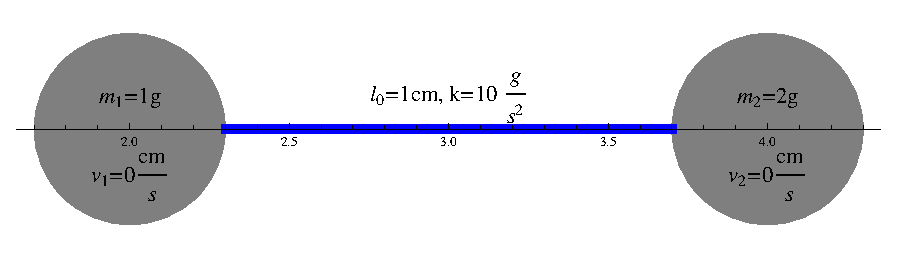
\includegraphics{ex09_gr1.eps}

\section*{Aufgabe 9.2}

Hooke{'}s Gesetz: \(F=k\left(l_0-l\right)\) mit Betrachtung der Richtung der Kraft:\\
\(\Rightarrow  F_1=k\left(l_0-\left\left| x_1-x_2\right\right| \right)*\frac{x_1-x_2}{\left\left| x_1-x_2\right\right| }=10\frac{g}{s^2}(1\text{cm}-\left|
2\text{cm}-4\text{cm}\right| )*\frac{2\text{cm}-4\text{cm}}{\left| 2\text{cm}-4\text{cm}\right| }=10\frac{g}{s^2}(-1\text{cm})*(-1)=10\text{cm} \frac{g}{s^2}\)\\
\(\Rightarrow  F_2=k\left(l_0-\left\left| x_2-x_1\right\right| \right)*\frac{x_2-x_1}{\left\left| x_2-x_1\right\right| }=10\frac{g}{s^2}(1\text{cm}-\left|
4\text{cm}-2\text{cm}\right| )*\frac{4\text{cm}-2\text{cm}}{\left| 4\text{cm}-2\text{cm}\right| }=10\frac{g}{s^2}(-1\text{cm})*1=-10\text{cm} \frac{g}{s^2}\)

\begin{doublespace}
\noindent\(\pmb{\text{Graphics}\left[\left\{\text{Gray},\text{Disk}[\{2,0\},0.3],\text{Disk}[\{4,0\},0.3], \text{Black},\text{Text}\left[\text{Style}\left[\texttt{"}m_1\text{=1g$\texttt{"}$},
\text{FontSize}\to 15\right], \{2,0.1\}\right], \right.\right.}\\
\pmb{\text{Text}\left[\text{Style}\left[\texttt{"}m_2\text{=2g$\texttt{"}$},\text{FontSize}\to 15\right], \{4,0.1\}\right], \text{Thickness}[0.01],
\text{Black}, \text{Text}\left[\text{Style}\left[\texttt{"}v_2\text{=0}\frac{\text{cm}}{s}\texttt{"}, \text{FontSize}\to 15\right], \{4,-0.15\}\right],}\\
\pmb{\text{Text}\left[\text{Style}\left[\texttt{"}v_1\text{=0}\frac{\text{cm}}{s}\texttt{"}, \text{FontSize}\to 15\right], \{2,-0.15\}\right], \text{Text}\left[\text{Style}\left[\texttt{"}l_0\text{=1cm,
k=10 }\frac{g}{s^2}\texttt{"}, \text{FontSize}\to 15\right], \{3,0.1\}\right], }\\
\pmb{\text{Text}\left[\text{Style}\left[\texttt{"}F_1\texttt{"}, \text{FontSize}\to 15\right], \{2.5,0.1\}\right],\text{Text}\left[\text{Style}\left[\texttt{"}F_2\texttt{"},
\text{FontSize}\to 15\right], \{3.5,0.1\}\right],\text{Red}, \text{Arrow}[\{\{2.3,0\},\{2.75,0\}\}], }\\
\pmb{\text{Arrow}[\{\{3.7,0\},\{3.25,0\}\}],\text{Blue}, \text{Dashed}, \text{Line}[\{\{2.3,0\},\{3.7,0\}\}]\}, \text{Axes}\to \{\text{True}, \text{False}\},
\text{AxesOrigin}\to \{0,0\},}\\
\pmb{\text{ImageSize}\to \text{Large}]}\)
\end{doublespace}

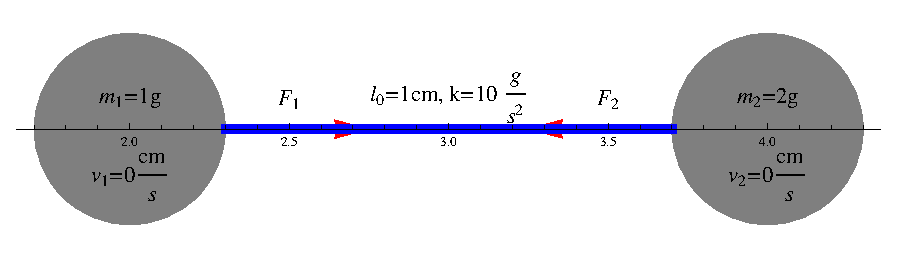
\includegraphics{ex09_gr2.eps}

\section*{Aufgabe 9.3}

\(x_1(t+h)=x_1(t)+h x_1'(t)=x_1(t)+h v_1(t)=2\text{cm} +1 s * 0\frac{\text{cm}}{s}=2\text{cm}\)\\
\(x_2(t+h)=x_2(t)+h x_2'(t)=x_2(t)+h v_2(t)=4\text{cm} +1 s * 0\frac{\text{cm}}{s}=4\text{cm}\)

\(a_1(t)=\frac{F_1}{m_1}=\frac{10\text{cm} *g}{s^2*1 g}=10 \frac{\text{cm}}{s^2}\)\\
\(a_2(t)=\frac{F_2}{m_2}=\frac{-10\text{cm} *g}{s^2*2 g}=-5 \frac{\text{cm}}{s^2}\)

\(v_1(t+h)=v_1(t)+h v_1'(t)=v_1(t)+h a_1(t)=0\frac{\text{cm}}{s}+1s*10\frac{\text{cm}}{s^2}=10\frac{\text{cm}}{s}\)\\
\(v_2(t+h)=v_2(t)+h v_2'(t)=v_2(t)+h a_2(t)=0\frac{\text{cm}}{s}+1s*-5\frac{\text{cm}}{s^2}=-5\frac{\text{cm}}{s}\)

Nicht stabil, da sich im n{\" a}chsten Schritt beide Kugeln durchdringen werden; kausal nicht erkl{\" a}rbar.

\section*{Aufgabe 9.4}

a)\\
Da hier auf jeden Fall: \(x_2>x_1\) gilt, k{\" o}nnen \(F_1 \text{und} F_2\) wie folgt vereinfacht werden:\\
\(F_1\left(x_1, x_2\right)=k\left(l_0-\left(-\left(x_1-x_2\right)\right)\right)*\frac{x_1-x_2}{-\left(x_1-x_2\right)}=-k\left(l_0+x_1-x_2\right)\)\\
\(F_2\left(x_1, x_2\right)=k\left(l_0-\left(x_2-x_1\right)\right)*\frac{x_2-x_1}{x_2-x_1}=k\left(l_0+x_1-x_2\right)\)

Damit ist die Jakobi-Matrix:\\
\(J=\left(
\begin{array}{cc}
 \frac{\partial F_1}{\partial x_1} & \frac{\partial F_1}{\partial x_2} \\
 \frac{\partial F_2}{\partial x_1} & \frac{\partial F_2}{\partial x_2} \\
\end{array}
\right)=\left(
\begin{array}{cc}
 -k & k \\
 k & -k \\
\end{array}
\right)\)

b)\\
\(\left(
\begin{array}{c}
 m_1a_1' \\
 m_2a_2' \\
\end{array}
\right)=\left(
\begin{array}{c}
 F_1 \\
 F_2 \\
\end{array}
\right)+h J \left(
\begin{array}{c}
 v_1 \\
 v_2 \\
\end{array}
\right)+h^2 J \left(
\begin{array}{c}
 a_1' \\
 a_2' \\
\end{array}
\right)=\left(
\begin{array}{c}
 10 \\
 -10 \\
\end{array}
\right)\text{cm}\frac{g}{s^2}+ 1 s * \left(
\begin{array}{cc}
 -10 & 10 \\
 10 & -10 \\
\end{array}
\right) \frac{g}{s^2}*\left(
\begin{array}{c}
 0 \\
 0 \\
\end{array}
\right)\frac{\text{cm}}{s}+ (1s)^2*\left(
\begin{array}{cc}
 -10 & 10 \\
 10 & -10 \\
\end{array}
\right) \frac{g}{s^2}\left(
\begin{array}{c}
 a_1' \\
 a_2' \\
\end{array}
\right)\\
\\
\unicode{29e6}\left(
\begin{array}{cc}
 1 & 0 \\
 0 & 2 \\
\end{array}
\right)\left(
\begin{array}{c}
 a_1' \\
 a_2' \\
\end{array}
\right)g=\left.\left(
\begin{array}{c}
 10 \\
 -10 \\
\end{array}
\right)\text{cm}\frac{g}{s^2}+\left(
\begin{array}{cc}
 -10 & 10 \\
 10 & -10 \\
\end{array}
\right) \left(
\begin{array}{c}
 a_1' \\
 a_2' \\
\end{array}
\right)g\text{  }\right| :g \left| - \left(
\begin{array}{cc}
 -10 & 10 \\
 10 & -10 \\
\end{array}
\right) \left(
\begin{array}{c}
 a_1' \\
 a_2' \\
\end{array}
\right)\right.\\
\\
\unicode{29e6}\left(
\begin{array}{c}
 10 \\
 -10 \\
\end{array}
\right)\frac{\text{cm}}{s^2}=\left(
\begin{array}{cc}
 11 & -10 \\
 -10 & 12 \\
\end{array}
\right)\left(
\begin{array}{c}
 a_1' \\
 a_2' \\
\end{array}
\right)\\
\\
\unicode{29e6}\left(
\begin{array}{c}
 a_1' \\
 a_2' \\
\end{array}
\right)=\left(
\begin{array}{cc}
 \frac{3}{8} & \frac{5}{16} \\
 \frac{5}{16} & \frac{11}{32} \\
\end{array}
\right)\left(
\begin{array}{c}
 10 \\
 -10 \\
\end{array}
\right)\frac{\text{cm}}{s^2}\\
\\
\unicode{29e6}\left(
\begin{array}{c}
 a_1' \\
 a_2' \\
\end{array}
\right)=\left(
\begin{array}{c}
 \frac{5}{8} \\
 -\frac{5}{16} \\
\end{array}
\right)\frac{\text{cm}}{s^2}\)

c)\\
\(\left(
\begin{array}{c}
 v_1' \\
 v_2' \\
\end{array}
\right)=\left(
\begin{array}{c}
 v_1 \\
 v_2 \\
\end{array}
\right)+h\left(
\begin{array}{c}
 a_1' \\
 a_2 \\
\end{array}
\right)=\left(
\begin{array}{c}
 0 \\
 0 \\
\end{array}
\right)\frac{\text{cm}}{s}+1s*\left(
\begin{array}{c}
 \frac{5}{8} \\
 -\frac{5}{16} \\
\end{array}
\right)\frac{\text{cm}}{s^2}=\left(
\begin{array}{c}
 \frac{5}{8} \\
 -\frac{5}{16} \\
\end{array}
\right)\frac{\text{cm}}{s}\)\\
\(\left(
\begin{array}{c}
 x_1' \\
 x_2' \\
\end{array}
\right)=\left(
\begin{array}{c}
 x_1 \\
 x_2 \\
\end{array}
\right)+h\left(
\begin{array}{c}
 v_1' \\
 v_2 \\
\end{array}
\right)=\left(
\begin{array}{c}
 2 \\
 4 \\
\end{array}
\right)\text{cm}+1s*\left(
\begin{array}{c}
 \frac{5}{8} \\
 -\frac{5}{16} \\
\end{array}
\right)\frac{\text{cm}}{s}=\left(
\begin{array}{c}
 \frac{21}{8} \\
 \frac{59}{16} \\
\end{array}
\right)\text{cm}=\left(
\begin{array}{c}
 2.625 \\
 3.6875 \\
\end{array}
\right)\text{cm}\)\\


\end{document}
